\section{Method}
\label{sec:method}

\begin{figure*}[t]
\centering
\setlength{\fboxsep}{5pt}
\small
\fbox{\parbox[c][1.0cm][c]{0.12\textwidth}{\centering RGB image\\or 4-frame clip}}
$\longrightarrow$
\fbox{\parbox[c][1.0cm][c]{0.15\textwidth}{\centering Frozen backbone\\V-JEPA 2.1 / DINOv3}}
$\longrightarrow$
\fbox{\parbox[c][1.0cm][c]{0.18\textwidth}{\centering Depth head\\linear / DPT / SFP / DTA}}
$\xrightarrow{\;h,K\;}$
\fbox{\parbox[c][1.0cm][c]{0.13\textwidth}{\centering FiLM or\\Pose-MVS}}
$\longrightarrow$
\fbox{\parbox[c][1.0cm][c]{0.12\textwidth}{\centering Metric depth\\and depth bins}}
$\longrightarrow$
\fbox{\parbox[c][1.0cm][c]{0.12\textwidth}{\centering 2D--3D lift\\SSC fusion}}
\caption{End-to-end study design. The backbone is frozen in every controlled depth experiment. RGB or video tokens feed a last-layer linear probe, a four-level dense decoder, or a temporally aligned decoder. Altitude $h$, intrinsics $K$, and calibrated poses enter only the explicitly marked conditioning/geometry paths. The resulting metric depth or depth distribution lifts image context into the OccuFly voxel grid before SSC fusion. This diagram separates backbone representation, depth recovery, geometric lifting, and semantic completion.}
\label{fig:end_to_end_overview}
\end{figure*}

We evaluate frozen V-JEPA~2.1 image and video features for two aerial 3D tasks: metric depth estimation and semantic scene completion (SSC). The framework is organized as a controlled sequence of probes and decoders. For MDE, we compare linear probing, DPT-style dense decoding, final-layer SFP adaptation, FiLM metadata conditioning, and video-token aggregation. For SSC, we use CGFormer- and FoundationSSC-inspired designs because their image-context and geometry pathways can be varied independently. This lets us isolate the contributions of frozen representation transfer, dense decoding, altitude/intrinsics conditioning, temporal aggregation, monocular depth priors, and pose-aware multiview geometry. Fig.~\ref{fig:evaluation_overview} summarizes the evaluation flow.

\begin{figure*}[t]
\centering
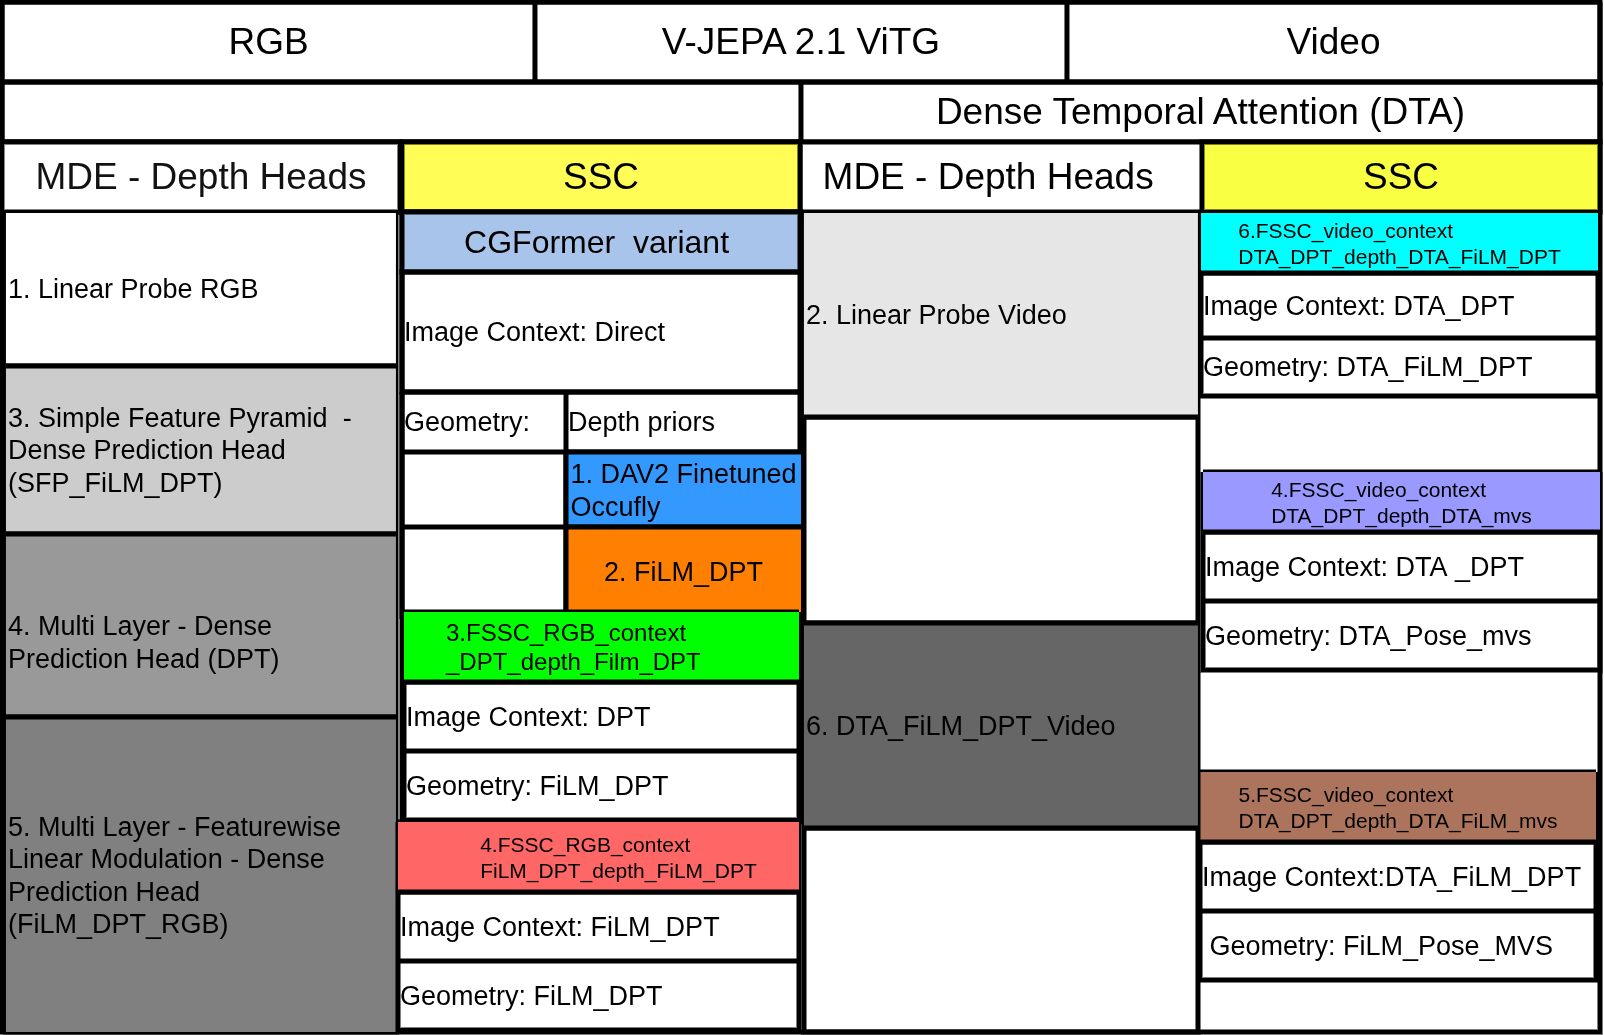
\includegraphics[width=\textwidth]{content/images/overview/ev.drawio.png}
\caption{Evaluation overview for the dense feature-transfer study. The figure summarizes the progression from frozen V-JEPA 2.1 RGB/video representations to monocular and multiview depth estimation heads, followed by the SSC variants that use the selected context and geometry pathways.}
\label{fig:evaluation_overview}
\end{figure*}

\subsection{Problem Formulation and Notation}
\label{sec:method_problem}

Each OccuFly sample is represented as
\begin{equation}
    s_t = \left(I_t, D_t, M_t, Y_t, K_t, h_t, T_t^{w\rightarrow c}\right),
\end{equation}
where $I_t \in \mathbb{R}^{3\times H\times W}$ is an RGB frame, $D_t$ is metric depth, $M_t \in \{0,1\}^{H\times W}$ is the valid-depth mask, $Y_t$ is the semantic occupancy grid, $K_t$ is the camera intrinsic matrix, $h_t$ is UAV altitude, and $T_t^{w\rightarrow c}\in\mathbb{R}^{4\times4}$ is the world-to-camera pose.

The monocular depth, pose-aware multiview depth, and SSC mappings are
\begin{equation}
    \begin{aligned}
    f_D^{\theta_D}&: (I_t,K_t,h_t) \mapsto \hat{D}_t,\\
    f_{D,\mathrm{MVS}}^{\theta_M}&: (\mathcal{V}_t,h_t)
        \mapsto (\hat{D}_t^{\mathrm{MVS}},P_t^{D,\mathrm{MVS}}),\\
    f_S^{\theta_S}&: (\Phi_t, K_t, h_t, \hat{D}_t, P_t^D) \mapsto \hat{Y}_t.
    \end{aligned}
    \label{eq:task_functions}
\end{equation}
The multiview input is
\begin{equation}
    \mathcal{V}_t =
    \left\{(I_{t_i},K_{t_i},T_{t_i}^{w\rightarrow c})\right\}_{i=0}^{N_s},
    \qquad t_0=t,
    \label{eq:mvs_view_set}
\end{equation}
where $t_0$ is the target view and $t_1,\ldots,t_{N_s}$ are calibrated source views. We use two views in this study. The V-JEPA~2.1 encoder is frozen in all experiments; trainable parameters are restricted to the depth heads $\theta_D$, MVS head $\theta_M$, and SSC modules $\theta_S$ according to the evaluated variant. $\Phi_t$ denotes the target visual context, $\hat{D}_t$ the dense metric depth estimate, $P_t^D$ the ray-wise depth probability tensor used for lifting, and $\hat{Y}_t$ the predicted semantic occupancy grid.

\subsection{Frozen V-JEPA 2.1 Feature Extraction}
\label{sec:method_vjepa_features}

Let $E_\theta$ be the frozen V-JEPA~2.1 encoder \cite{murlabadia2026vjepa21}. For the ViT-Gigantic checkpoint used here, the input resolution is $384\times384$, patch size is 16, the spatial grid is $24\times24$, the feature dimension is $C=1664$, and the 48 transformer blocks are indexed from 0 to 47.

\paragraph{RGB mode.}
For a target frame $I_t$, we use either the final feature map or four intermediate layers,
\begin{equation}
    \mathcal{L}_{\mathrm{G}}=\{11,23,37,47\},
    \qquad
    F_t^{(l)} = E_{\theta}^{(l)}(I_t)\in\mathbb{R}^{1664\times24\times24},
    \quad l\in\mathcal{L}_{\mathrm{G}}.
    \label{eq:vjepa_multilayer_features}
\end{equation}
The linear probe uses only $F_t^{(47)}$. The DPT variants consume selected intermediate maps and reassemble them into multiscale dense features following DPT \cite{ranftl2021dpt}.

\begin{figure}[t]
\centering
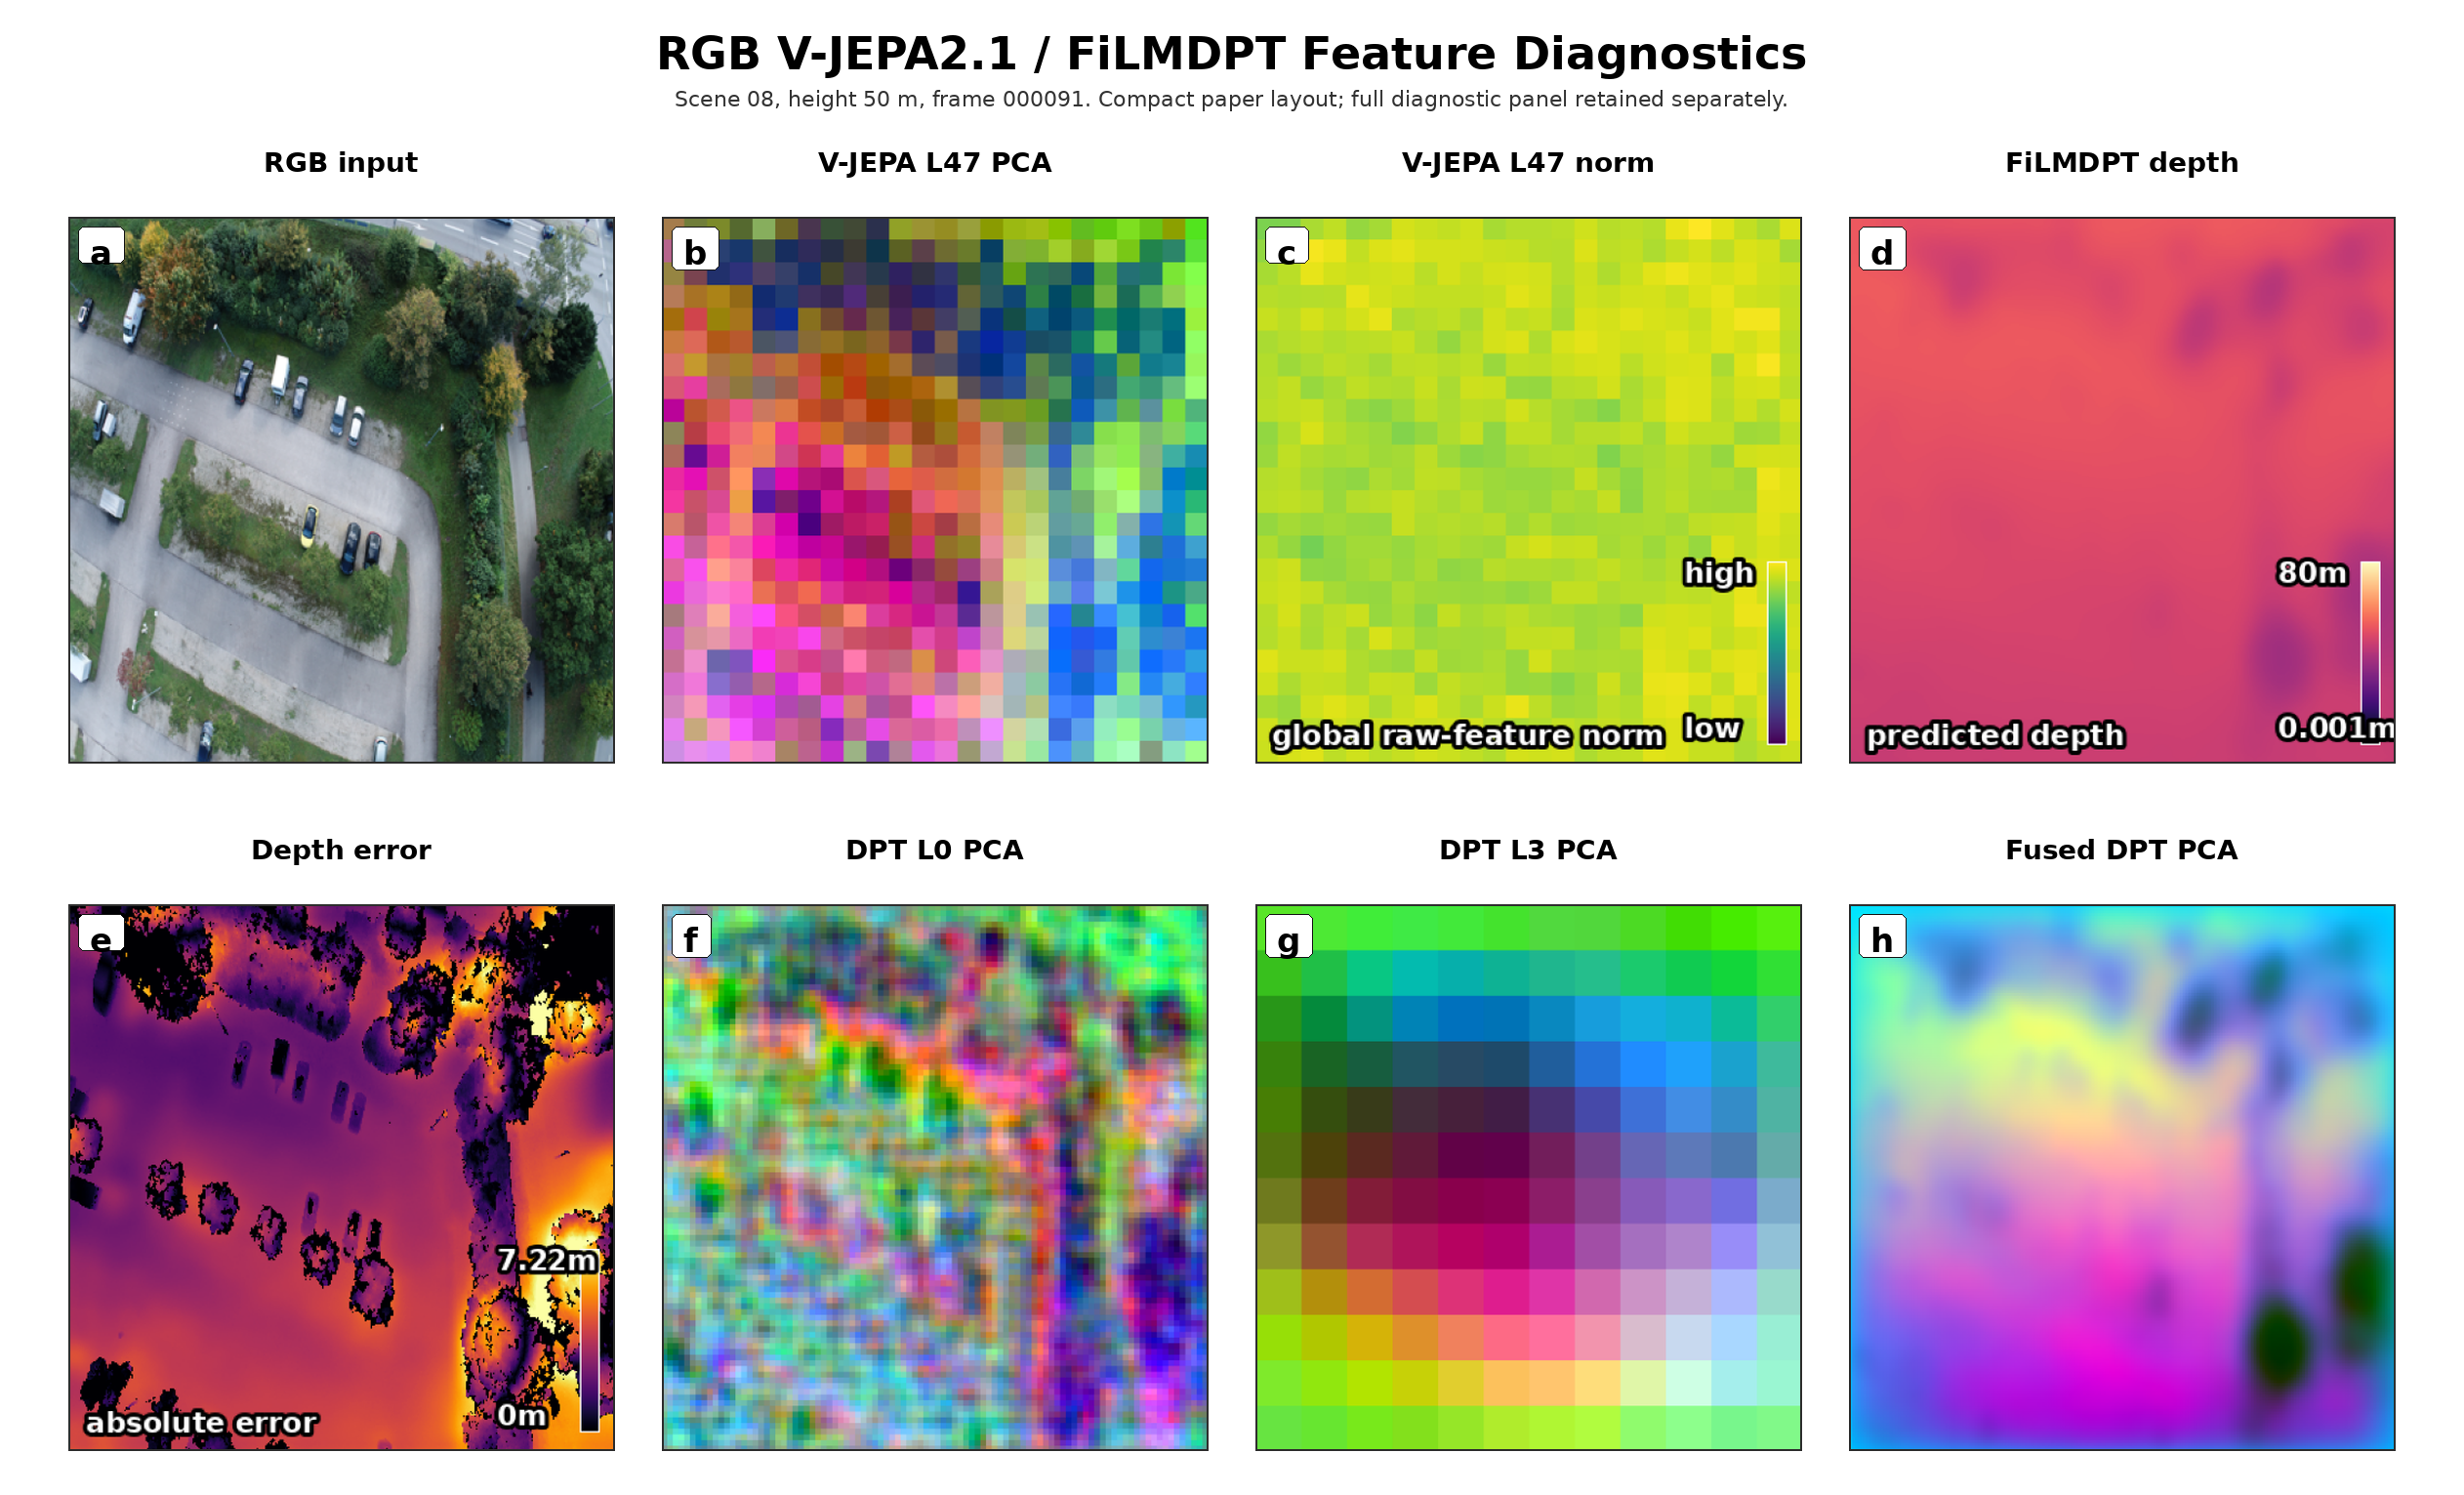
\includegraphics[width=0.82\linewidth]{content/images/vjepargbvideo_token_transfer/rgb_final_layer_pca_norm_filmdpt_panel.png}
\caption{Compact RGB V-JEPA~2.1/FiLM-DPT feature diagnostic. PCA views of frozen and decoder-processed features illustrate spatially organized cues used by downstream dense prediction.}
\label{fig:vjepa_rgb_feature_diagnostics}
\end{figure}

\paragraph{Video mode.}
We form a four-frame target-centered clip
\begin{equation}
    \begin{gathered}
    X_t = [I_{t+\tau_1}, I_{t+\tau_2}, I_{t+\tau_3}, I_{t+\tau_4}]
    \in \mathbb{R}^{3\times4\times384\times384},\\
    [\tau_1,\tau_2,\tau_3,\tau_4]=[-1,0,0,+1].
    \end{gathered}
\end{equation}
The duplicated zero offset keeps the clip target-centered while matching the V-JEPA~2.1 tubelet size. Because the OccuFly preprocess files used here do not include capture timestamps, temporal neighborhoods are defined by frame offset rather than physical time.

For tubelet size 2, the four-frame clip produces $T'=2$ temporal tubelet positions:
\begin{equation}
    G_t^{(l)} = E_{\theta}^{(l)}(X_t)
    \in \mathbb{R}^{1664\times T'\times24\times24}.
    \label{eq:vjepa_video_features}
\end{equation}
We test two adapters. The video linear probe folds the tubelet axis into channels,
\begin{equation}
    \begin{gathered}
    G_t^{(47)}\in\mathbb{R}^{1664\times T'\times24\times24}
    \mapsto
    \widetilde{F}_t\in\mathbb{R}^{(1664T')\times24\times24},\\
    \widetilde{F}_t[t'C+c,u,v]=G_t^{(47)}[c,t',u,v].
    \end{gathered}
    \label{eq:video_linear_probe_fold}
\end{equation}
For $T=4$, $\widetilde{F}_t\in\mathbb{R}^{3328\times24\times24}$.

The Dense Temporal Attention (DTA) adapter converts video tokens into target-frame maps. For each $l\in\{11,23,37,47\}$ and spatial location $(u,v)$, temporal descriptors are
\begin{equation}
    S_{t,u,v}^{(l)}=
    [G_t^{(l)}[:,1,u,v],\ldots,G_t^{(l)}[:,T',u,v]]
    \in \mathbb{R}^{T'\times1664}.
\end{equation}
A lightweight learned-query attention block returns one feature vector per spatial cell,
\begin{equation}
    \bar{F}_t^{(l)}[:,u,v]=
    \mu_t^{(l)}[:,u,v]
    +\alpha_l\left(\mathrm{DTA}_l(S_{t,u,v}^{(l)})-\mu_t^{(l)}[:,u,v]\right),
    \label{eq:dta_residual}
\end{equation}
where $\mu_t^{(l)}=\operatorname{mean}_{\tau}G_t^{(l)}[:,\tau,:,:]$ and the residual gate $\alpha_l$ is initialized near mean pooling. The maps $\{\bar{F}_t^{(l)}\}$ then have the same $1664\times24\times24$ form as RGB maps and can be passed to the DPT, feature-to-depth, or pose-aware MVS modules.

\begin{figure*}[t]
\centering
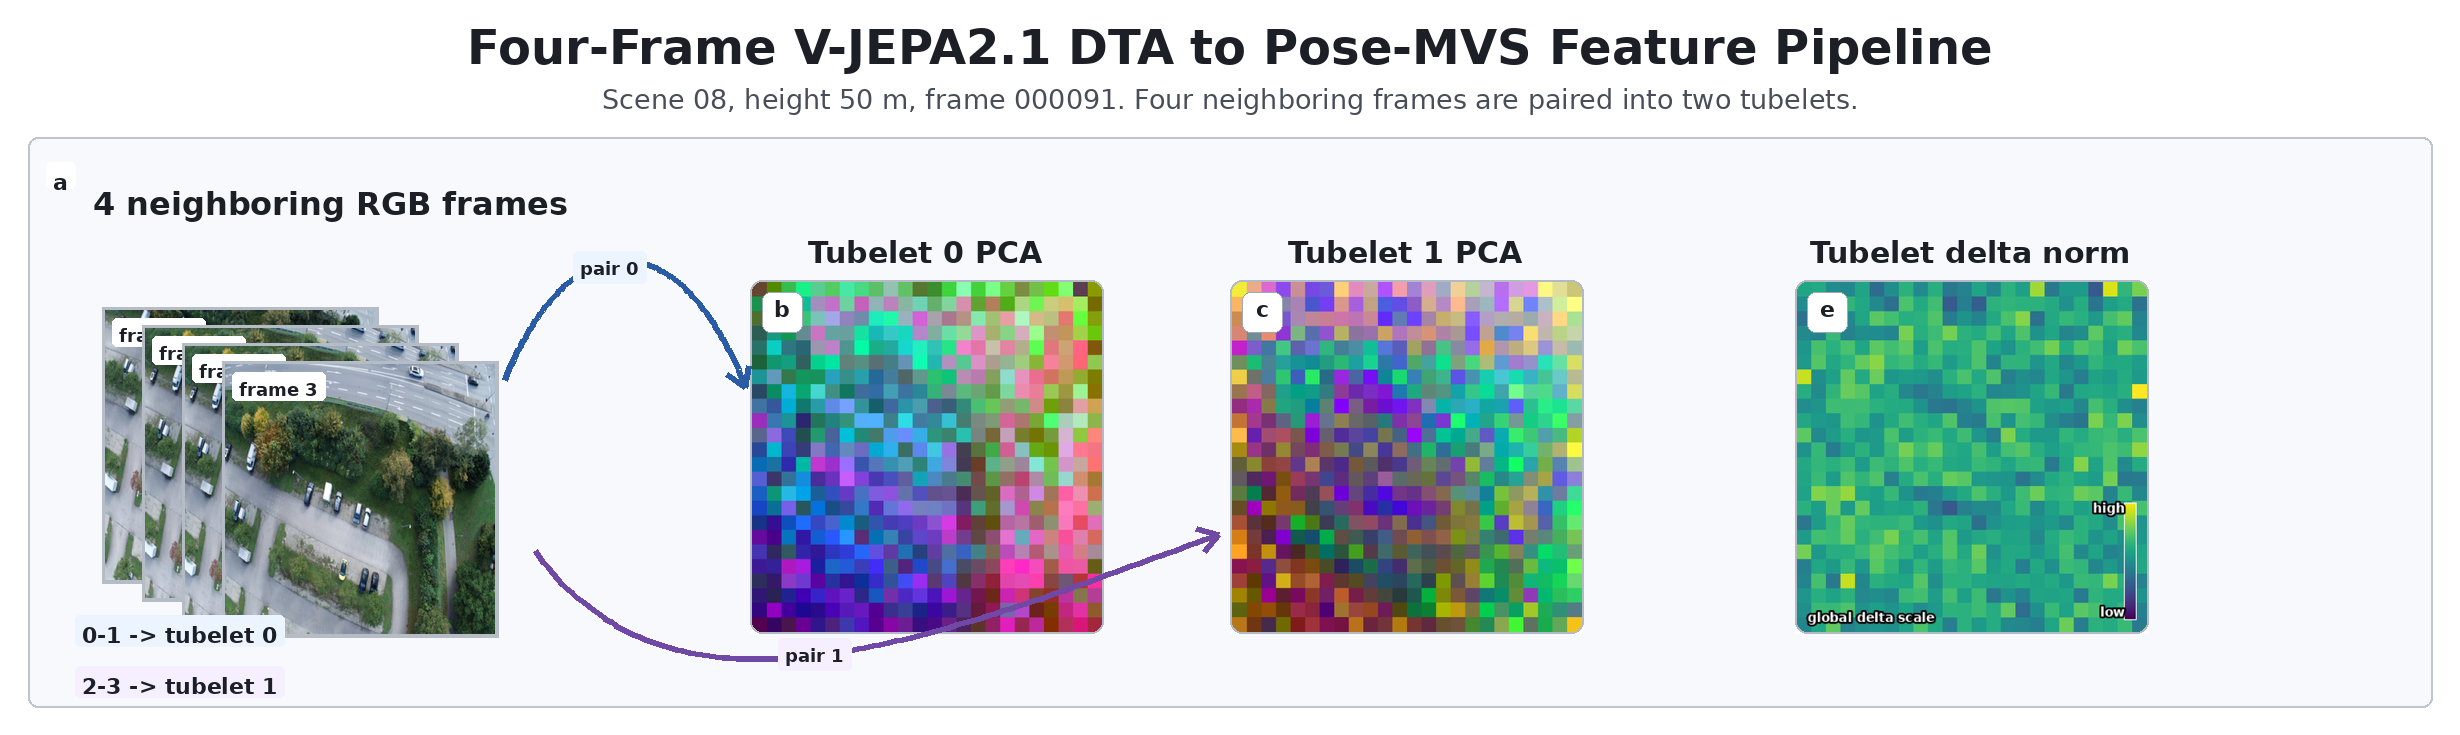
\includegraphics[width=0.86\textwidth]{content/images/vjepargbvideo_token_transfer/vjepavideotokens.png}
\caption{Compact video-token diagnostic for the four-frame V-JEPA~2.1 pathway. Consecutive RGB frames form two tubelet positions whose PCA projections and feature-delta norm summarize the temporal cues exposed to DTA and pose-aware MVS modules.}
\label{fig:vjepa_video_token_diagnostics}
\end{figure*}

\subsection{Depth Estimation}
\label{sec:method_depth_heads}

All depth heads predict logits over $K_D=256$ metric depth bins and convert them to a dense expectation,
\begin{equation}
    p_{k,u,v}=\operatorname{softmax}_k(z_{k,u,v}),
    \qquad
    \hat{D}_{u,v}=\sum_{k=1}^{K_D}p_{k,u,v}d_k,
    \label{eq:depth_estimate}
\end{equation}
where $d_k$ are bin centers. Monocular heads produce $z$ from linear or DPT-style decoders; Pose-MVS produces $z$ from a regularized projective cost volume.

\begin{figure}[t]
\centering
\fbox{\begin{tabular}{ll}
\textbf{Input split} & OccuFly train/validation/test samples \\
$\downarrow$ & image $(I_t,K_t,h_t)$, video clip $(X_t,K_t,h_t)$, \\
& or posed views $\mathcal{V}_t$ \\
\textbf{Frozen backbone} & V-JEPA 2.1 features $F_t^{(l)}$ or $G_t^{(l)}$ \\
$\downarrow$ & LP / SFP-DPT / DPT-FiLM / Video-FiLM-DPT \\
& / Pose-MVS-FiLM \\
\textbf{Trainable head} & depth-bin logits \\
$\downarrow$ & \\
\textbf{Output} & depth probabilities $P_t^D$ and estimated depth $\hat{D}_t$ \\
& or MVS counterparts $(P_t^{D,\mathrm{MVS}},\hat{D}_t^{\mathrm{MVS}})$
\end{tabular}}
\caption{Common depth-estimation flow. The V-JEPA 2.1 backbone is frozen, while the depth head is trained on the official OccuFly train/validation/test split.}
\label{fig:depth_flow}
\end{figure}

\begin{table*}[t]
\centering
\definecolor{trainpink}{RGB}{255,225,235}
\newcommand{\trainable}[1]{\mbox{\setlength{\fboxsep}{1pt}\colorbox{trainpink}{\ensuremath{#1}}}}
\caption{Simplified component flow for the depth-head variants. Light-pink boxes denote the learnable components updated during training; unmarked V-JEPA 2.1 feature extraction remains frozen.}
\label{tab:depth_block_flows}
\begin{tabular}{p{0.19\linewidth}p{0.73\linewidth}}
\toprule
\textbf{Variant} & \textbf{Data flow with representative shapes} \\
\midrule
RGB Linear Probe &
$I_t\rightarrow F_t^{(47)}[1664,24,24]\rightarrow \trainable{\mathrm{BN}+1{\times}1}\rightarrow Z_t[256,24,24]\rightarrow(\hat{D}_t,P_t^D)$. \\
\addlinespace
Video Linear Probe &
$X_t\rightarrow G_t^{(47)}[1664,T',24,24]\rightarrow \widetilde{F}_t[(1664T'),24,24]\rightarrow \trainable{\mathrm{BN}+1{\times}1}\rightarrow Z_t[256,24,24]\rightarrow(\hat{D}_t,P_t^D)$. \\
\addlinespace
SFP-DPT &
$\begin{aligned}[t]
I_t&\rightarrow F_t^{(47)}[1664,24,24]\rightarrow \trainable{\mathrm{SFP}}\{S_4,S_2,S_1,S_{1/2}\}\\
&\rightarrow\trainable{\mathrm{DPT}}\rightarrow(\hat{D}_t,P_t^D),\\
S_\cdot&\in\{[256,96,96],[256,48,48],[256,24,24],[256,12,12]\}.
\end{aligned}$ \\
\addlinespace
DPT &
$I_t\rightarrow\{F_t^{(11)},F_t^{(23)},F_t^{(37)},F_t^{(47)}\}\rightarrow\trainable{\mathrm{DPT\ reassembly/fusion}}\rightarrow(\hat{D}_t,P_t^D)$. \\
\addlinespace
FiLM-DPT &
$I_t,K_t,h_t\rightarrow\{R_l\},e_t\rightarrow\trainable{\mathrm{FiLM}}(\{R_l\},e_t)\rightarrow\trainable{\mathrm{DPT\ fusion}}\rightarrow(\hat{D}_t,P_t^D)$. \\
\addlinespace
Video FiLM-DPT &
$X_t,K_t,h_t\rightarrow\{G_t^{(l)}\}\rightarrow\trainable{\mathrm{DTA}}\rightarrow\{\bar{F}_t^{(l)}\},e_t\rightarrow\trainable{\mathrm{FiLM\mbox{-}DPT}}\rightarrow(\hat{D}_t,P_t^D)$. \\
\addlinespace
Pose-MVS-FiLM &
$\mathcal{V}_t,h_t\rightarrow G_i^{(l)}\rightarrow\trainable{\mathrm{DTA}}\rightarrow\trainable{\mathrm{pose\ cost\ volume}}\rightarrow\trainable{\mathrm{FiLM\ logits}}\rightarrow(\hat{D}_t^{\mathrm{MVS}},P_t^{D,\mathrm{MVS}})$. \\
\bottomrule
\end{tabular}
\end{table*}

\paragraph{Linear probes.}
The RGB and video linear probes test whether metric aerial depth is directly accessible from frozen final-layer features. The RGB probe uses $F_t^{(47)}$; the video probe uses $\widetilde{F}_t$ from Eq.~\eqref{eq:video_linear_probe_fold}. Both use only a batch-normalized $1\times1$ prediction head, following dense frozen-feature probing practice \cite{simeoni2025dinov3,facebookresearch_dinov3_linear_head}.

\subsubsection{DPT Depth Decoders}
\label{sec:method_dpt_decoders}

DPT-style decoders reassemble transformer maps into image-like features and fuse them with convolutional refinement \cite{ranftl2021dpt}. For selected layers,
\begin{equation}
    R_l = \rho_l\left(F_t^{(l)}\right),
    \qquad R_l\in\mathbb{R}^{C_D\times H_l\times W_l},
    \quad C_D=256,
    \label{eq:dpt_reassembly}
\end{equation}
where $\rho_l$ is the DPT reassembly/projection block. The maps are either fused directly or FiLM-conditioned before fusion.

\paragraph{SFP-DPT.}
The SFP variant tests whether the final V-JEPA~2.1 feature map can serve as a dense multiscale source without intermediate layers. Inspired by the Simple Feature Pyramid used with plain ViTs in ViTDet \cite{li2022vitdet}, it constructs
\begin{equation}
    \operatorname{SFP}(F_t^{(47)})=
    \{S_4,S_2,S_1,S_{1/2}\},
    \qquad
    S_s\in\mathbb{R}^{256\times(24s)\times(24s)},
    \quad s\in\{4,2,1,1/2\}.
    \label{eq:sfp}
\end{equation}
The resulting pyramid is decoded by the same DPT-style depth head.

\paragraph{FiLM-conditioned DPT.}
\label{sec:method_dpt_film}
FiLM variants test whether altitude and camera calibration should modulate the frozen-feature decoder. The normalized metadata vector is
\begin{equation}
    m_t=\left[
    \frac{h_t-40}{10},\frac{f_x}{W},\frac{f_y}{H},\frac{c_x}{W}-0.5,\frac{c_y}{H}-0.5
    \right]\in\mathbb{R}^{5},
    \label{eq:metadata_vector}
\end{equation}
which a small MLP maps to $e_t\in\mathbb{R}^{128}$. For each DPT level,
\begin{equation}
    \widetilde{R}_l = R_l\odot\left(1+\gamma_l(e_t)\right)+\beta_l(e_t),
    \label{eq:film}
\end{equation}
where $\gamma_l$ and $\beta_l$ are channel-wise affine projections broadcast spatially. They are initialized near zero so the decoder starts close to the unconditioned DPT path. For video FiLM-DPT, DTA first converts tubelet features to $\{\bar{F}_t^{(l)}\}$; the same FiLM-DPT decoder is then applied. Equivalently, at each spatial site,
\begin{equation}
    \bar{F}_{t}^{(l)}(:,u,v)=
    \mu_{t}^{(l)}(:,u,v)
    +\alpha\left(\operatorname{Expand}\left(\operatorname{MLP}\left(\operatorname{MHA}(q,K,V)\right)\right)
    -\mu_{t}^{(l)}(:,u,v)\right),
    \label{eq:dta}
\end{equation}
with $\alpha=\sigma(a)$ initialized to approximately $0.1$.

\subsubsection{Pose-MVS-FiLM}
\label{sec:method_depth_pose_mvs_film}

Pose-MVS-FiLM constructs a depth-indexed cost volume from calibrated target/source views, following learned MVS cost-volume matching \cite{yao2018mvsnet}. For target pixel $\mathbf{u}=(u,v,1)^\top$ and depth-bin center $d_k$,
\begin{equation}
    \mathbf{x}_{t,k,u,v}=d_k K_t^{-1}\mathbf{u},
    \qquad
    \mathbf{q}_{i,k,u,v}=\pi\!\left(K_i T_{t\rightarrow i}
    \begin{bmatrix}\mathbf{x}_{t,k,u,v}\\1\end{bmatrix}\right),
    \label{eq:mvs_projection}
\end{equation}
where $\pi(\cdot)$ is perspective projection. Let $A_t$ and $A_i$ be target/source feature maps after video adaptation. Source features are sampled at projected coordinates and aggregated over source views,
\begin{equation}
    \widetilde{A}_{i,k,u,v}=\operatorname{sample}\left(A_i,\mathbf{q}_{i,k,u,v}\right),
    \qquad
    C_{t,k,u,v}=\operatorname{Agg}_{i\in\mathcal{S}_t}
    \operatorname{corr}\left(A_t(:,u,v),\widetilde{A}_{i,k,u,v}\right).
    \label{eq:mvs_cost_volume}
\end{equation}
A 3D CNN regularizes $C_t$ and produces FiLM-conditioned depth logits,
\begin{equation}
    \begin{gathered}
    Z_{t}^{\mathrm{MVS}}=\phi_{\mathrm{logit}}\!\left(\psi_{3\mathrm{D}}(C_t),e_t\right),\\
    P_{t}^{D,\mathrm{MVS}}=\operatorname{softmax}_k Z_t^{\mathrm{MVS}},
    \qquad
    \hat{D}_{t,u,v}^{\mathrm{MVS}}=\sum_{k=1}^{K_D}P_{t,k,u,v}^{D,\mathrm{MVS}}d_k .
    \end{gathered}
    \label{eq:mvs_depth_estimate}
\end{equation}
This branch uses the same 256 depth-bin centers and target-frame depth supervision as Eq.~\eqref{eq:depth_estimate}.

\begin{table*}[t]
\centering
\caption{Depth-estimation variants and the transfer question isolated by each design. Learnable components are shown in Table~\ref{tab:depth_block_flows}.}
\label{tab:method_depth_variants}
\begin{tabular}{p{0.26\linewidth}p{0.65\linewidth}}
\toprule
\textbf{Variant} & \textbf{Purpose} \\
\midrule
Linear probe & Tests whether metric aerial depth is linearly accessible from frozen V-JEPA 2.1 features. \\
SFP-DPT & Tests whether the final V-JEPA 2.1 map can be converted into an effective dense pyramid without intermediate layers. \\
DPT & Tests whether selected intermediate layers improve dense metric depth over final-layer probing. \\
FiLM-DPT & Tests whether altitude/intrinsics conditioning improves RGB or video depth decoding. \\
Pose-MVS-FiLM & Tests whether calibrated multiview matching and metadata conditioning improve the geometric prior. \\
\bottomrule
\end{tabular}
\end{table*}

\subsubsection{Altitude-Interpolation Depth Evaluation}
\label{sec:method_altitude_interpolation_depth}

The standard OccuFly split uses scenes 01--05 for training, scenes 06--07 for validation, and scenes 08--09 for testing, with altitudes 30, 40, and 50~m. We also evaluate altitude interpolation: training uses 30 and 50~m samples from scenes 01--08, validation uses 40~m samples from scenes 01--04, and testing uses 40~m samples from scenes 05--08,
\begin{align}
    \mathcal{D}_{\mathrm{train}} & = \{s_t: h_t\in\{30,50\},\ \operatorname{scene}(t)\in\{01,\ldots,08\}\}, \\
    \mathcal{D}_{\mathrm{val}} & \subset \{s_t: h_t=40,\ \operatorname{scene}(t)\in\{01,02,03,04\}\}, \\
    \mathcal{D}_{\mathrm{test}} & \subset \{s_t: h_t=40,\ \operatorname{scene}(t)\in\{05,06,07,08\}\}.
\end{align}
This split tests whether FiLM conditioning supports metric scale interpolation rather than only fitting observed flight heights.

\subsection{Semantic Scene Completion}
\label{sec:method_ssc}
\label{sec:method_depth_probabilities}

\begin{wrapfigure}[20]{r}{0.52\linewidth}
\vspace{-1.0em}
\centering
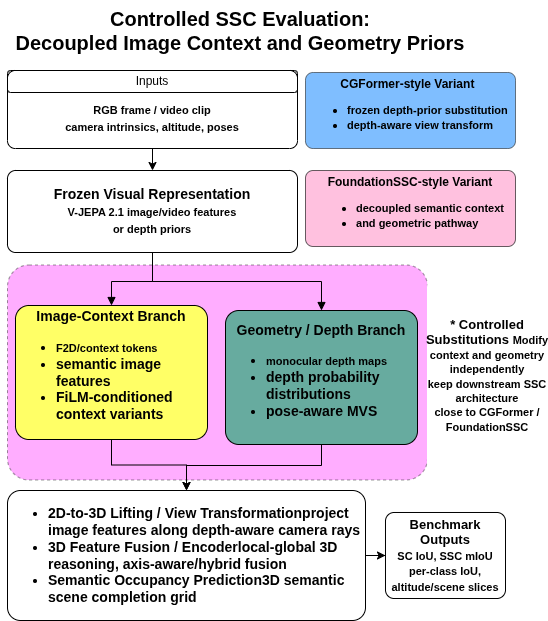
\includegraphics[width=\linewidth,trim=6 11 0 0,clip]{content/images/overview/ssc_p.drawio.png}
\caption{Conceptual SSC flow with independently varied image-context and geometry-depth pathways.}
\label{fig:ssc_decoupled_context_geometry_flow}
\vspace{-1.0em}
\end{wrapfigure}

The SSC benchmark separates image context from geometry. The context pathway provides semantic visual features; the geometry pathway provides monocular depth, depth probabilities, or pose-aware MVS priors. Both are lifted into a common 3D representation before fusion and semantic occupancy prediction. The goal is not to introduce a completely new SSC architecture, but to use architectures whose exposed pathways support controlled feature-transfer studies.
